%%%%%%%%%%%%%%%%%%%%%%%%%%%%%%%%%%%%%%%%%%%%%%%%%%%%%%%%%%%%%%%%%%%%%%%%
% Plantilla TFG/TFM
% Escuela Politécnica Superior de la Universidad de Alicante
% Realizado por: Jose Manuel Requena Plens
% Contacto: info@jmrplens.com / Telegram:@jmrplens
%%%%%%%%%%%%%%%%%%%%%%%%%%%%%%%%%%%%%%%%%%%%%%%%%%%%%%%%%%%%%%%%%%%%%%%%

\chapter{State of Art}
\label{marcoteorico}
As we previously stated, semantic segmentation is a extremely important task in the field of computer vision due to it's value towards complete scene understanding.
In this section we will review some of the most common and recent deep network architectures, data-sets and frameworks that tackle the semantic segmentation problem.

\section{Introduction}
Before we dive into the next sections it is important to understand semantic segmentation and where it comes from. Semantic segmentation is a natural evolution of the object recognition problem, the goal is to infer the class for every pixel on the image, obtaining a pixel-by-pixel labeled image
. 
Semantic segmentation is not so different from classic object recognition, in fact it's fundamentally the same, it just adds an extra layer of complexity towards the more fine-grained solutions. We could go further and try to differentiate instances of the same class, that would be instance segmentation. \todo{image recognition grain figure}

\section{Sim 2 Real}
In the last decade, data driven algorithms have vastly surpassed traditional techniques for computer vision problems, these algorithms, although can be tuned and improved in many different ways, still require vast amounts of quality, precisely annotated data in order to yield good results. In the real world environment, there are quite a few limitations to the quantity and quality of the data that can be produced. For instance, we could be limited to the number of cameras and annotators, moving physical objects to setup scenes could also be difficult and time consuming, and dangerous situations could be risky to set up properly i.e trying to get an autonomous car to learn to avoid pedestrians when there is no time to brake.
    
Sim2Real is a specific section of the data science field that mainly focuses on the automatic generation and ground-truth annotation of synthetic data by simulating the real world in a virtual environment. Although a virtual environment will allow us to workaround the previously mentioned restrictions, there's still a reality gap that must be covered in order for the synthetic data to be transferred to real life situations. Most synthetic data scenarios will present discrepancies between them and the real-world, to overcome this and properly transfer the knowledge to real problems there are two known approaches that have been proven to be effective. The first one and probably the most obvious is to generate extremely realistic environments, to achieve this multiple techniques can be applied, such as rendering very high and photo-realistic textures, models and lightning or simulating the noise of real cameras by applying filters and post-process effects. The other method, domain randomization \cite{DBLP:journals/corr/TobinFRSZA17} which is based on showing the model a huge amount of different synthetic data, with this method even if the data is not extremely accurate to real data, the variability of the multiple range of data will make up for it and the model will learn.

In this section we will review some of the latest works on the field.

\subsection{VirtualHome}
VirtualHome is a three dimensional environment built in the Unity game engine. The main goal is to model complex tasks in a household environment as sequences of more atomic and simple instructions.
 
In order to perform this task a big database describing activities composed by multiple atomic steps was necessary, in the human natural language there is a lot of information that is common knowledge and is usually omitted, however, for a robot or agent this information has to be provided in order to fully understand. For this purpose an interface to formalize this tasks was built on top of the Scratch \footnote{\url{https://scratch.mit.edu/}} MIT project. Then all of this atomic actions and interactions were implemented using the Unity3D game engine.

For the data collection, they had workers describe in natural language all of these tasks and then built them using the Scratch interface. Every task is composed by a sequence of steps where every step is a Scratch block, and every block defines a syntactic frame and a list of arguments for the different interactions that they may have.

Every step $t$ in the program can be written as:

\[ step_t = [action_t] (object_{t,1})(id_{t,1}) ... (object_{t,n})(id_{t,n}) \]

Where id is an identifier to differentiate instances of the same object. An example program to "watch tv" would look like this: 
\newline

$step_1$ = [Walk] (TELEVISION)(1)

$step_2$ = [SwitchOn] (TELEVISION)(1)

$step_3$ = [Walk] (SOFA)(1)

$step_4$ = [Sit] (SOFA)(1)

$step_5$ = [Watch] (TELEVISION)(1) \newline

\subsection{UnrealROX}
UnrealROX \cite{DBLP:journals/corr/abs-1810-06936} is a photo-realistic 3D virtual environment built in \gls{ue4} capable of generating synthetic, ground-truth annotated data.

\section{Common Arquitectures}
As we previously stated, semantic segmentation is a natural step towards the more fine-grained image recognition problem, since the information that we are trying to infer is higher level, we will also require more complex architectures. Although the models we will be reviewing in this section work properly for image recognition and detection, some modifications will have to be made in order to adapt them for segmentation problems. However, they have made such significant contributions to the field that they are still being used as the basic building blocks segmentation architectures.

\subsection{AlexNet}
AlexNet was the first deep network architecture that successfully surpassed traditional machine learning approaches, winning the \gls{ilsvrc} 2012 with a 84.6\% TOP-5 test accuracy, easily surpassing the its competitors by a huge margin. The architecture itself was pretty straight forward. It consisted of five convolution + pooling layers followed by three fully connected ones as seen in figure \ref{alexnet}.


\begin{figure}
	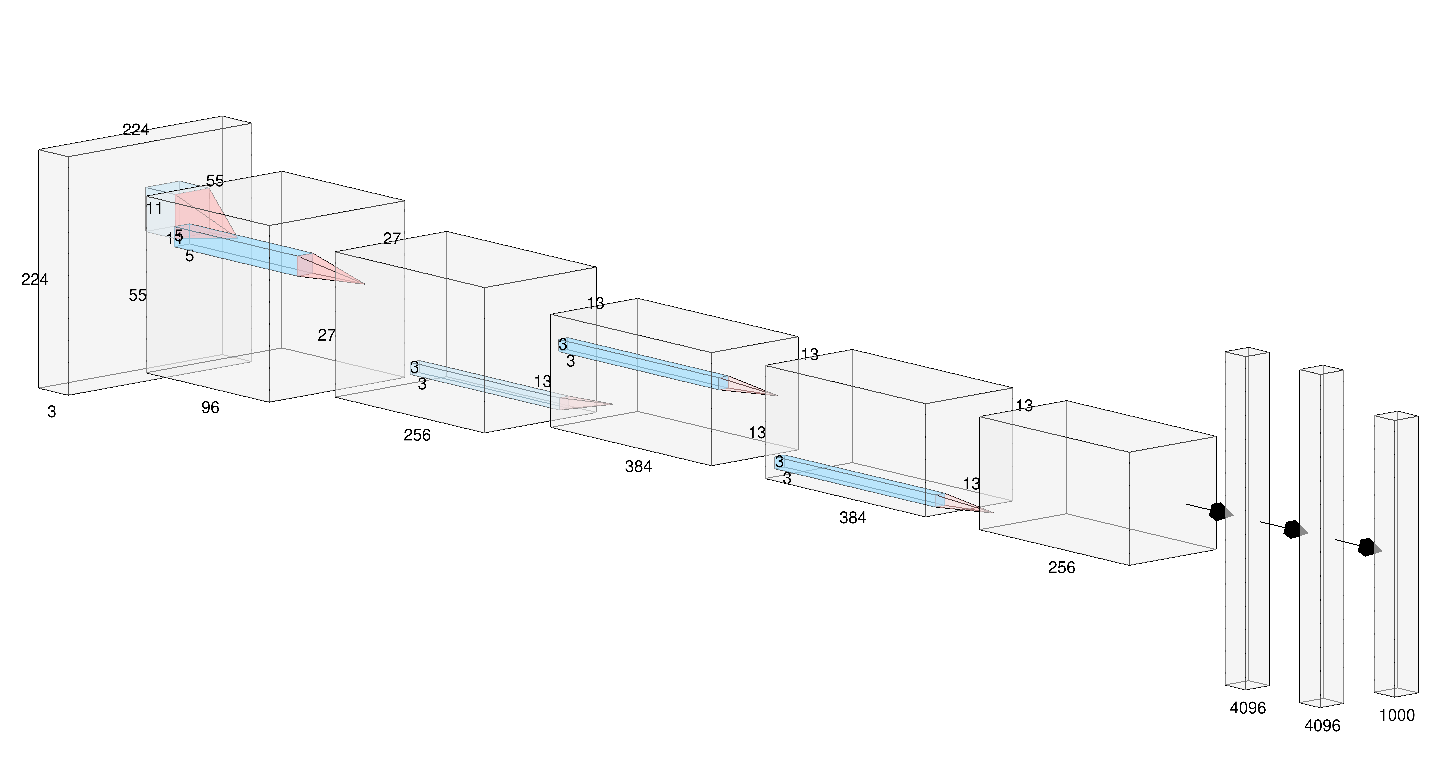
\includegraphics[scale=0.3]{archivos/alexnet.png}
	\centering
	\caption{AlexNet architecture reproduced from \cite{AlexNet}}
	\label{alexnet}
\end{figure}

\subsection{VGG}
VGG is also a deep network model introduced by the \gls{vgg}, one of the various model configurations proposed \cite{DBLP:journals/corr/SimonyanZ14a} was submitted to the \gls{ilsvrc} 2013. The VGG-16 achieved 92.7\% TOP-5 test accuracy.

\subsection{GoogLeNet}
GoogLeNet (also known as Inception) was introduced by (cite) and was submitted to \gls{ilsvrc} 2014, winning with a TOP-5 test accuracy of 93.3\%. GoogLeNet architecture is rather complex, it introduced the inception module (shown in figure \ref{inception}) which consisted of a new approach where convolution layers were not stacked in just sequential order but instead had some of them compute in parallel, which substantially reduced computational cost.

\begin{figure}
	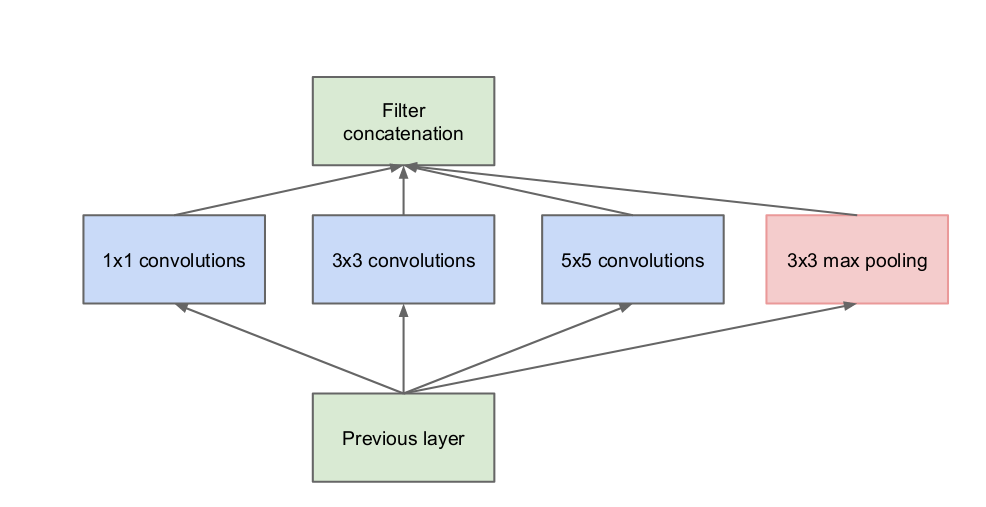
\includegraphics[scale=0.3]{archivos/inception_module.png}
	\centering
	\caption{Inception module extracted from \cite{DBLP:journals/corr/SzegedyLJSRAEVR14}}
	\label{inception}
\end{figure}

\subsection{ResNet}
ResNet was first introduced by Microsoft research and it got very popular after achieving 96.4\% in \gls{ilsvrc} 2016. This \gls{cnn} is extremely deep with 152 layers and it introduced a new concept called residual blocks (figure), this new module allowed the network inputs to skip layers and copy them to deeper layers, and so the compute output is a combination of X and F(X) as seen in (figure). This allows for deeper but also less computationally demanding networks.

\subsection{ReNet}
Multi Dimensional Recurrent Neural Network (MDRNN) are a variation of regular RNN that allow them to work with $d$ spatio-temporal dimensions of the data. The architecture proposed by (cite) used regular RNN instead of MDRNN, where every convolution + pooling layer is replaced by four RNN's that sweep the image across in four directions. 

\subsection{Semantic Segmentation Variants}
All the image recognition problem solutions based on convolutional architectures, whether it is recognition, detection, localization or segmentation, they all share a big common module, which is the convolution layers that will extract the features of any image, after that we can adapt our network for our specific problem.

Today, almost every semantic segmentation architecture uses the \gls{fcn} by \cite{DBLP:journals/corr/LongSD14}. The idea behind this is to replace the fully connected layers of previously well known architectures for image classification such as ResNet or GoogleNet with \gls{fcn} in order to obtain a spatial map instead classification outputs, this way we can obtain pixel-wise classification while still using the inferred knowledge and power of the \gls{cnn}'s. Convolutional layers (convolution + pooling) downsample the input image in order to learn features, this downsampling does not matter when applied to classification problems, however, when doing pixel-wise classification, we require the output image to have the same size as the input. To overcome this problem, spatial maps are then upsampled by using deconvolution layers as shown in \cite{deconvolution}.

\subsubsection{Decoder Variant}
The decoder variant is another method to adapt networks that were initially made for classification. In this variant, the network after removing the fully connected layers is normally called encoder and it outputs a low-resolution feature map. The second part of this variant is called decoder and the main idea behind it is to up-sample those feature maps to obtain a full resolution pixel-wise classification.

A very good example of this encoder-decoder architecture is SegNet \cite{DBLP:journals/corr/BadrinarayananK15}, encoder part is fundamentally the same as a \gls{vgg}-16 without the fully connected layers at the very end, while the decoder part consists of a combination of convolution and upsampling layers that correspond to the max-pooling ones in the encoder.

  
\section{Datasets}
In this section we will review some of the most important datasets that are commonly used to train semantic segmentation architectures. 

\subsection{PASCAL}
PASCAL Visual Object Classes is one of the most popular 2D datasets for semantic segmentation. The challenge consists of 5 different competitions, 21 ground-truth annotated classes and a private test set to verify the accuracy of submitted models. Also there are a few extensions of this dataset such as PASCAL Context or PASCAL Part.

\subsection{Semantic Boundaries Dataset}
This dataset is an extension of the PASCAL dataset that provides semantic segmentation ground-truth annotations for all the images that were not labeled in the original dataset. SBD greatly increases the amount of data from the original PASCAL and because of this is commonly used for deep learning architectures.

\subsection{Cityscapes}
Cityscapes is a urban dataset mainly used for instance and semantic segmentation. It contains over 25000 images and 30 different classes was recorded in 50 cities during different times of the day and year.

\subsection{KITTI}


